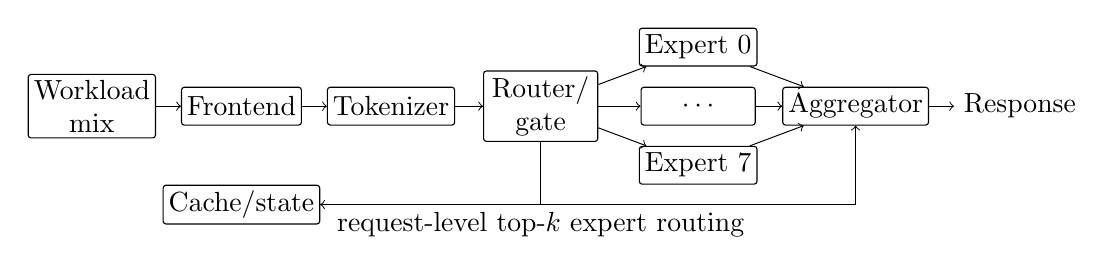
\begin{tikzpicture}[
svc/.style={draw, rounded corners=1pt, align=center, minimum width=1.45cm,
minimum height=0.48cm, inner sep=2pt},
edge/.style={->, line width=0.35pt}
]
\node[svc] (load) at (0,0) {Workload\\mix};
\node[svc] (front) at (1.9,0) {Frontend};
\node[svc] (tok) at (3.8,0) {Tokenizer};
\node[svc] (router) at (5.7,0) {Router/\\gate};
\node[svc] (expert0) at (7.7,0.75) {Expert 0};
\node[svc] (expertd) at (7.7,0) {\(\cdots\)};
\node[svc] (expert7) at (7.7,-0.75) {Expert 7};
\node[svc] (agg) at (9.7,0) {Aggregator};
\node[svc] (cache) at (1.9,-1.25) {Cache/state};

\draw[edge] (load) -- (front);
\draw[edge] (front) -- (tok);
\draw[edge] (tok) -- (router);
\draw[edge] (router) -- (expert0);
\draw[edge] (router) -- (expertd);
\draw[edge] (router) -- (expert7);
\draw[edge] (expert0) -- (agg);
\draw[edge] (expertd) -- (agg);
\draw[edge] (expert7) -- (agg);
\draw[edge] (router) |- (cache);
\draw[edge] (cache) -| (agg);
\draw[edge] (agg) -- ++(1.25,0) node[right] {Response};
\node[align=center] at (5.7,-1.5) {request-level top-\(k\) expert routing};
\end{tikzpicture}
